
\documentclass[12pt, letterpaper]{article}
\usepackage{hyperref}
\usepackage[utf8]{inputenc}
\usepackage{amsfonts}
\usepackage{amsmath}
\usepackage{lwarp-titlesec}
\usepackage{graphicx}
\graphicspath{\Schule\Physik\graphics}
\hypersetup{
    colorlinks=true,
    linkcolor=blue,
    filecolor=magenta,      
    urlcolor=cyan,
    pdftitle={Overleaf Example},
    pdfpagemode=FullScreen,
    }

\title{Physik, Goldbach}
\author{Aaron Tsamaltoupis}


\begin{document}
\maketitle
\tableofcontents
\newpage

\begin{document}
\section{Elektrische Felder}
\label{sec:Elektrische Felder}
\index{Elektrische Felder}
Es gibt zwei Ladungsarten: 
\begin{itemize}
  \item negative Elektrische Ladungen\item positive Elektrische Ladungen
\end{itemize}
Ein negativ geladener Körper weist einen Elektronenüberschuss, ein positiv geladener Körper einen Elektronenmangel auf.
\subsection{Influenz}
\label{sec:Influenz}
Influenz: ausgelöst durch elektrisches oder magnetisches feld, kann zu Polarisation führen
\section{Doppler effekt}
\index{Doppler effekt}
Die Frequenzaenderung, die man beim Vorbeifahren einer Schallquelle wahrnimmt heisst dopplereffekt.\\\\
Beispiele:\\
-Naehern/Entfernen eines Krankenwagens\\\\
\subsection{Bewegte Quelle}
\begin{math}
    \lambda_{Beobachter} = \lambda_{Quelle} - v\cdot T\\
    \frac{c}{f_{beobachter}}=\frac{c}{f_{quelle}}-v\cdot \frac{1}{f_{quelle}} |:c\\
    \frac{1}{f_{beobachter}}=\frac{1}{f_{quelle}}-\frac{v}{c}\cdot \frac{1}{f_quelle}\\
    \frac{1}{f_{beobachter}}=\frac{1}{f_{quelle}}\cdot (1-\frac{v}{c})\\\\
    \Rightarrow f_{beobachter = \frac{1}{1-\frac{v}{c}}}
\end{math}
\\\\
-Wenn die Quelle auf den Beobachter zukommt, dann ist v positiv\\
$\Rightarrow 1-\frac{v}{c}<1$\\
$\Rightarrow f_{beobachter} > f_{quelle}$\\
-Wenn die Quelle sich von dem Beobachter entfernt, dann ist v negativ:
\begin{math}
    \Rightarrow 1-\frac{v}{c}>1\\
    \Rightarrow f_{beobacter} < f_{quelle}\\
\end{math}
Die wahrgenommene Tonfrequenz ist tiefer
wenn 
\begin{math}
    v=0 \Rightarrow f_{beobachter}=f_{quelle}
\end{math}
\subsection{Bewegter Beobachter}
\begin{math}
    f_{beobachter} = \frac{c+v}{\lambda} = f_{quelle}\cdot \frac{c+v}{c} = (1+\frac{v}{c})\cdot f_{quelle}
\end{math}


\section{Der Lichtelektrische Effekt (Fotoeffekt)}
\index{Lichtelektrischer Effekt}
Durchfuehrung:\\
  Eine mit einem Elektroskop verbundene Zinkplatte
  \begin{enumerate}
    \item wird negativ geladen.
    \item wird negativ geladen und eine Glasplatte wird davor gehalten
      \item wird positiv geladen.
  \end{enumerate}
  Anschliessend wird die Zinkplatte mit einer Lampe mit hohem UV-Licht Anteil bestrahlt.\\\\
Beobachtung:\\
\begin{enumerate}
  \item Zunaechst schlaegt das Elektroskop aus, nach der Bestrahlung entlaedt sich das Elektroskop
  \item Das Elektroskop schlaegt aus, entlaedt sich aber nicht nach Bestrahlung
  \item Das Elektroskop entlaedt sich nicht nach der Bestrahlung
  \item im Falle einer ungeladenen Zink-Platte ist ebenfalls keine Veraenderung zu beobachten.
  \item Mit zunehmender LIchtintensitaet steigt die Fotostromstaerke
\end{enumerate}
Ergebnis:\\
Wird eine Metallschicht mit Licht bestrahlt, koennen aus dem Metall Elektronen herausgeloest werden.\\
Das Ausloesen von Elektronen durch Lichtbestrahlung bezeichnet man als \textit{Lichtelektrischen Effekt}  oder \textit{Fotoeffekt}. \\
Voraussetzung fuer den Fotoeffekt ist eine \textit{Mindestfrequenz} des eingestrahlten Lichts.\\\\
Erklaerung:\\
Zum Herausloesen von Elektronen aus einem Metallr muss \textit{Austrittsarbeit}  verrichtet werden.\\
Die kinetische Energie einzelner sich im Metallgitter frei bewegender Elektronen wird beim Auftreffen von Licht einer Mindestfrequenz soweit erhoeht, dass sie den Gitterverband gerade verlassen koennen.
Ist die Frequenz groesser als die Grenzfrequenz $f_{0}$, liegt die ueberschuessige Energie als zusaetzliche Energie der \textit{Fotoelektronen}  vor, es ist also ein \textit{Fotostrom} messbar.\\\\
\begin{math}
  W_{Licht} = W_{a} + W_{kin} 
\end{math}\\\\
Messung der kinetischen Energie der Fotoelektronen mit der sog. \textit{Gegenfeldmethode} :
\\Messprinzip: \\
Die Energie der gemessenen Fotospannung ist gleich der kinetischen Energie, die von der ueberschuessigen Energie der Lichtenergie uebrig geblieben ist.\\
$W_{el}= W_{kin}$\\
$W_{el} = e\cdot U$\\
$e\cdot U = W_{kin} = W_{Licht}-W_{a}$\\\\

Die Lichtenergie $W_{Licht}$ ist proportional zur Frequenz $f$, wobei die Konstante $h$ der Proportionalitaetsfaktor ist:\\$
$W_{Licht} = h\cdot f$\\
h: Plancksches Wirkungsquantum
$h=4,196\cdot 10^{-15}$\\
Die kinetische Energie der Fotoelektronen steigt linear mit der Frequenz des eingestrahlten Lichts:\\
$W_{kin} = h\cdot f-W_{a}$


\subsection{Fotoeffekt Zusammenfassung}
Zusammenfassung der experimentellen Befunde:
\begin{enumerate}
  \item Licht mit zu niedriger Freuquenz (zu grosser Wellenlänge) löst keine Elektronen aus einer Metallschicht aus.
  \item Die kinetische Energie der Fotoelektronen stiegt linear mit der Frequenz des Eingestrahlten Lichts: \\ 
    \begin{math}
      W_{kin, max}=hf-W_a\\
      W_a = hf_{grenz}
    \end{math}\\
    $f_{grenz}$ \textit{ist die frequenz, wo elektronen gerade so herausgelöst werden, ohne dass zusätzliche kinetische Energie freigesetzt wird} \\
  \item Die Stärke des Fotostroms ist der Lichtintensität \textit{proportional} 
  \item Bei konstanter Frequenz ist die (maximale) kinetische Energie der Fotoelektronen unabhängig von der Lichtintensität.\\
    \\
\begin{math}
  Lichtintensität = \frac{auftreffende Lichtenergie}{Zeit*Fläche} 
  \index{Lichtintensität}
  
\end{math}
\item Die Fotoelektronen werden bei Bestrahlung spontan aus dem Metallgitter herausgelöst
\end{enumerate}
\subsection{Lichtquantenhypothese nach Albert Einstein}
Bei der Ausbreitung von Licht ist die Energie nicht kontinuiertlich über den Raum verteilt, sondern in einer endlichen Zahl von Energiequanten lokalisiert. Licht ist ein strom von Lichtquanten oder Photonen, die sich mit Lichtgeschwindigkeit bewegen, unteilbar sind und nur als Ganzes erzeugt oder absorbiert werden können.\\
In monochromatischem Licht der Frequnz f tr'gt jedes Lichqant die Energie: $W_{Licht}=h \cdot f$\\
$h= 6,626 Js$ (\textit{Plancksches Wirkungsquantum}  \\
\index{Plancksches Wirkungsquantum}

eEine Erhöhung der Intensität des Lichts bedeutet eine Vergrößerung der Anzahl der pro Zeiteinheit auftretenden Lichtquanten, nicht aber das Auftreten von energiereicheren Quanten.\\
Je nach dem Matrerial, indem sie sich befinden, benötigen Elektronen ein Minimum an Energie um aus dem Material gelöst zu werden. Diese Energie muss sich aber in dem einzelnen Photonen befinden und kann nicht als Summe der Energie der Lichtintensität über einen Zeitraum zu den Elektronen befördert werden.\\
Die Zeit bis das minimum an Lichtenergie erreicht ist, ist also irrelevant, das Elektron kann nur direkt, \textit{spontan}, von einem Photon mit genug Energie gelöst werden. 
\newpage
\section{Exkurs: Äquivalenz von Masse und Energie}
\label{sec:Exkurs: Äquivalenz von Masse und Energie}

berechnete Masse von Helium Kern:
$m_{He-Kern} = 2\cdot m_{p}+2\cdot m_{n}\approx 6,695\cdot 10^{27}}$
tatsächliche Masse von Herlium Kern:
$m_{He-Kern}=4,001228U$\\\\
Feststellung: Die tatsächliche Masse des Helium-Kerns ist geringer als die Summe der Massen aller Nukleonen (Protonen, Neutronen)\\
Informationen: nach Einstein sind Energie und Mase zueinander äquivalente Grössen.\\
Die bei der "Enstehung" des He-Kerns verschwundenen Masse ist als Energie freigeworden.\\\\

Masse und Impuls eines Photons
\index{Masse, Impuls eines Photons}
\\\begin{math}
  E=mc^{2}=W_{photon} = h\cdot f\\
  m_{photon} = \frac{h\cdot f}{c^{2}} 
\end{math}\\
Damit hat das Photon den Impuls $P_{Photon =m_{photon} \cdot  c = \frac{h\cdot f}{ c^{2}} \cdot c}}$\\
P_{Photon = \frac{h\cdot f}{c} =\frac{h}{\lambda} }

\newpage
\section{Elektronenwellen}
\subsection{Elektronenwellen - die Hypothesen um de Broglie}
\index{Elektronenwellen, De Broglie}

\begin{enumerate}
  \item Die Ausbreitung eines jeden Teilchens erfolgt als Welle, deren Wellenlängedurch $\lambda = \frac{h}{p} $ gegeben ist
  \item Zwichen der Freqenz der Wellen und der Gesamtenergie W des Teilchen besteht die Beziehung $W = h \cdot f$

\end{enumerate}
\subsubsection{Abschätzung der Wellenlänge der Elektronenwelle}
\label{sec:elektronenwellen}
sei  $U=3kV$\\
\begin{math}
  W_{kin}=W_{el}=e\cdot U\\
  W_{kin}= \frac{1}{2} c\cdot m_{e}v^2 = e\cdot U\\\\
  v^2 = \frac{e\cdot 2U}{m_{e}} 
  \\\\
  v= \sqrt{\frac{ec\cdot 2U}{m_{e}} } \\\\
  p = m_{e}\cdot v : berechnet\ den\ Impuls\\\\
  \lambda = \frac{h}{p} = \frac{h}{m_{e}\cdot v} \\\\
  \lambda = \frac{h}{m\cdot \sqrt{\frac{e\cdot 2U}{m_{e}} }}= \frac{h}{m\cdot \sqrt{\frac{2e\cdot 3000V}{m_{e}} }}  = 2,24 \cdot 10^{-11}m = 22,4 pm\ (Größenbereich\ Gammastrahlen)
\end{math}
\newpage
\subsection{Einschub: Bragg-Reflexionen}
Versuch: Hinter der Öffnung einer Lochanode einer Elektronenstrahlröhre befindet sich eine Folie mit Grahpit
pulver.\\
Beobachtung: Auf dem Leuchtschirm sind um den hellsten Punkt in der Mitte Ringe von heller und weniger heller Leuchtintensität zu sehen.\\
\\
\textbf{Röntgenstrahlung trifft auf einen (Dreh)Kristall}\\ 
\\



Beobachtung:\\
Versuche zeigen, ass man nur unter ganz bestimmten Einfalls- und damit Reflexionswinkeln eine besonders hohe Inteinsität der reflektierten Wellen misst, bei anderen Einfallswinkeln ist die Intensität  der reflektierten Wellen fast null. \\ 
Diese Erscheinung heisst Bragg-Reflexion.
\\\\
Gangunterschied = $\Delta s=2d\cdot sin(\alpha)$\\
Ein Maximum entsteht dort, wo die Bedingung für kontstruktive Interferenz erfüllt ist: \\
generell gilt:\\
\begin{math}
 wenn\ \Delta s = k\cdot \lambda\ dann\ konstruktive\ Differenz
\end{math}\\
sei $2d\cdot sin(\alpha_{0})= k\cdot \lambda$
\\Jeder Winkel für den dies gilt ist ein sog Glanzwinkel $\alpha_{glanz}$
\\Glanzwinkel sind also die Winkeln, bei denen es zu kontstruktiver Interferenz kommt\\\\\\\\
\newpage
Die Interferenzringe entstehen folgendernmassen:\\
Die Graphitschicht enthaelt viele kleine Mikrokristalle. Unter ihnen gibt es immer einige, die gerade so liegen, dass die Elektronenstrahlung sie unter dem Glanzwinkel trifft.\\\\
Bragg-Gleichung:\\ $\Delta s =n\cdot \lambda = 2d\cdot sin(\alpha_{glanz})$\\
$tan(2\alpha_{glanz}) = \frac{R}{L} $\\
fuer kleine Winkel gilt:\\
$tan(2\alpha_{glanz}) \approx sin(2\alpha_{glanz})\approx 2\cdot sin(\alpha_{glanz})$\\\\
$\Rightarrow 2d\cdot  sin(\alpha_{glanz})\approx d\cdot  tan(2\alpha_{glanz})=d\cdot \frac{R}{L} $\\
$\Rightarrow n\cdot \lambda \approx d\cdot  \frac{R}{L} $\\\\
Beispiel:
\begin{enumerate}
  
  \item Wellenlaenge berechnet mit innerem Ring:\\$L=1,235$\\
$d_{1} = 2,13\cdot  10^{-10}m\ (Graphit)$\\
  
Radius R des inneren Rings bei $U=3kV: R_{i}= 0.0145m$\\
$\Rightarrow n=1$(\textit{ weil beobachteter Ring ist Maximum 1. Ordnung: innerster Ring gemessen, Reflexion des Elektronenstrahl von aeusserster Netzebene})\\\\
$\lambda= d_{1}\cdot \frac{R}{L}= 2,13\cdot 10^{-10}m\cdot  \frac{0,0145m}{0,135m} \approx 2,29\cdot 10^{-11}=22,9pm$\\\\
\textit{Die quantitativve Auswertung des Interferenzmusters bestaetigt die de-Broglie-Wellenlaenge von 22,4pm (siehe oben: \hyperref[sec:elektronenwellen]{Wellenlaenge De Broglie})}
 


\item Wellenlaenge berechnet mit auesserem Ring:\\ $L=1,235$\\
Radius R des auesseren Rings bei $U=3kV: R_{a} = 0.025m$\\
$\Rightarrow n=1$ \textit{(bei gleichbleibender Wellenlaenge $\lambda$ muss auch der aeussere Ring ein Maximum 1. Ordnung sein, siehe unten)}\\
$d_{2} = 1,23\cdot 10^{-10}m$\\
$\lambda=22.78\cdot 10^{-11}m = 22,78pm$\\

Die beiden hellen Ringe stellen also beide Maxima 1.Ordnung dar, die durch Interferenz der, je nach Lage des Kristalls, an den beiden moeglichen Ebenen des Waabenartig aufgebauten Grafitgitters reflektierten Elektronenwellen entstehen.
\end{enumerate}


\subsection{Quantenobjekte}
\index{Quantenobjekte}
\label{sec:Quantenobjekte}
Photonen, aber auch Elektronen, Neutronen, Protonen, Atome und Moleküle , nennt man Quantenobjekte.\\
Das Verhalten einzelner Quantenobjekte kann (in der Regel) nicht vorausgesagt (=determiniert) werden.\\
\textit{Quantenobjekte sind weder Teilchen noch Wellen.}\\

Bei einer geringen Anzahl an Quantenobjekten enstehen Auftereffverteilungn, die keine Ähnlichkeit mit dem Interferenzmuster der Optik haben. Je mehr Quantenobjekte aber z.B. den Doppelspalt durchlaufen, desto zuverlässiger tritt das Interfernezmuster auf.


\subsection{Wesenszüge von Quantenobjekten}
\index{Quantenobjekte, Wesenszüge}
\label{sec:Wesenszüge von Quantenobjekten}

\begin{enumerate}
  \item \textbf{Wesenszug 1: Statistisches Verhalten}
  \begin{itemize}
  \item Für Quantenobjekte können Einzelereignisse im Allgemeinen nicht vorhergesagt werden
  \item Bei vielen Wiederholungen ergibt sich jedoch eine Verteilung, die -bis auf stochastische Schwankungen- reproduzierbar ist.
  \end{itemize}
\item \textbf{Wesenszug 2: Fähigkeit zur Interferenz}
  \begin{itemize}
    
    \item Auch einzelne Quantenobjekte können zu einem Interferenzmuster beitragen.
  Voraussetzung ist, dass es für das Eintreten des gleichen Versuchsergebnisses mehr als eine klassisch denkbare Möglichkeit gibt.
\item \textsc{Erläuterung:}\\
  Beim Doppelspalt bedeutet dies, dass ein Photon durch Spalt 1 (Möglichkeit1) oder durch Spalt 2 (Möglichkeit 2) zum Schirmpunkt P gelangt. Das Ergebnis des Versuchs, der Nachweis eines Photons am Schirmpunkt P, ist in beiden Fällen das Gleiche.
  \end{itemize}
\item \textbf{Wesenszug 3: Eindeutige Messergebnisse} 
  \begin{itemize}
    \item Messergebnisse sind stets eindeutig, auch wenn sich das Quantenobjekt vor der Messung in einem Zustand befindet, der unbestimmt bezüglich der gemessenen Größe ist.
    \item \textsc{Erläuterung:}\\ Hinter dem Doppelspalt ist eine genaue Ortsmessung für ein Photon bzw. Elektron mölgich (vlg. Wesenszug 4). Vor der Messung war der Ort des Elektrons nicht bekannt. Man sagt dazu auch: Die Elektronen besaßen die Eigenschaft "Ort" nicht.
  \end{itemize}
\item \textbf{ Wesenszug 4: Komplementarität}
  \begin{itemize}
    \item Interferenzmuster und Unterscheidbarkeit der klassisch denkbaren Möglichkeiten schließen sich aus.
  \item \textsc{Erläuterung:}\\Bezogen auf den Doppelspalt bedeutet "Unterscheidbarkeit der klassisch denkbaren Möglichkeiten": man weiß durch eine geeignete Vorrichtung, ob das Quantenobjekt durch Spalt1 oder Spalt2 gegangenist. Allerdings verschwindet dann das Interferenzmuster. Ortseigenschaft und Interferenzmuster sind nicht gleichzeitig realisierbar, sondern schließen sich gegenseitig aus. Dies ist ein Spezialfall eines allgemeinen Prinzips, das man nach Niels Bohr \textit{Komplementarität}  nennt.
    
  \end{itemize}
\end{enumerate}

\newpage
\section{Atomphysik}
\label{sec:Atomphysik}
\index{Atomphysik}
\subsection{Energistufen in Atomen}
\label{sec:Energistufen in Atomen}
\textit{Durchführung: Beobachtung von verschiedenen Lampen durch Gitter}	\\
Beobachtungen:
\begin{enumerate}
\item	eine Glühlape oder eine Kerzenflamme senden ein kontinuierliches Spektrum aus.
\item Hg-Dampf-Lampe, eine Hz-Spektralröhre oder eine Na-Dampf-Lampe senden jeweils ein für sie charakterisches Linienspektrum aus, d.h. sie emittiert Licht mit für sie charakteristischen Frequenzen.\\
	\textit{Jeder Leuchtdampf sendet quanten mit bestimmten frequenzen}
Bei der Spektralanalyse wird ein LInienspektrum zum Nachweis von Stoffen genutzt.
\item Eine mit Natriumchlorid(NaCl) gefärbte Flamme wirft einen Schatten im LIcht einer Na-Dampf-Lampe, nicht aber im Licht einer Hg-Dampf-Lampe.
\end{enumerate}
\newpage
\textsc{Erklärung Verusch}	\\
\begin{enumerate}
  \item Na-Atome, Hg-Atome bzw. Hg-Atome emittieren im sichtbaren Bereich Lichtquanten mit für sie charakteristischer Energie $W_{licht} =h\cdot f=h\cdot \frac{c}{\lambda}	$
    	\begin{center}
    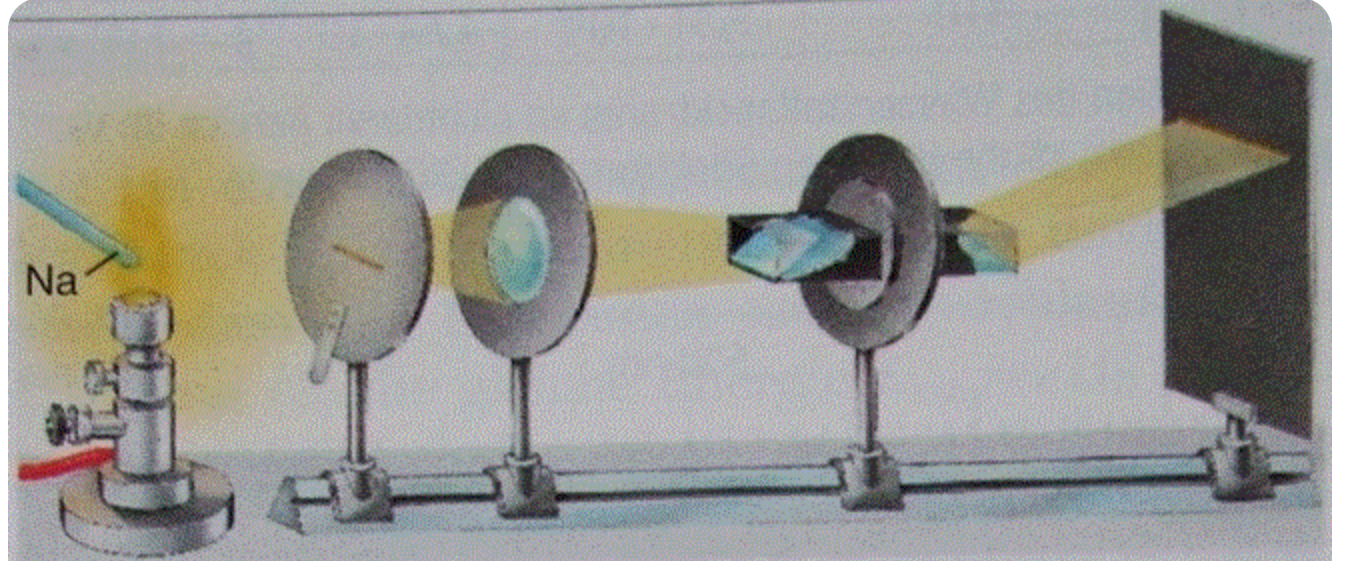
\includegraphics[width = 8cm]{graphics/IMG_0919.PNG}
    \end{center}
  \item Nur Lichtquanten von genau gleichen, für sie charakteristischen Betrag werden von Atomen auch absorbiert \textit{(Resonanzabsorption)}	
    	\begin{center}
    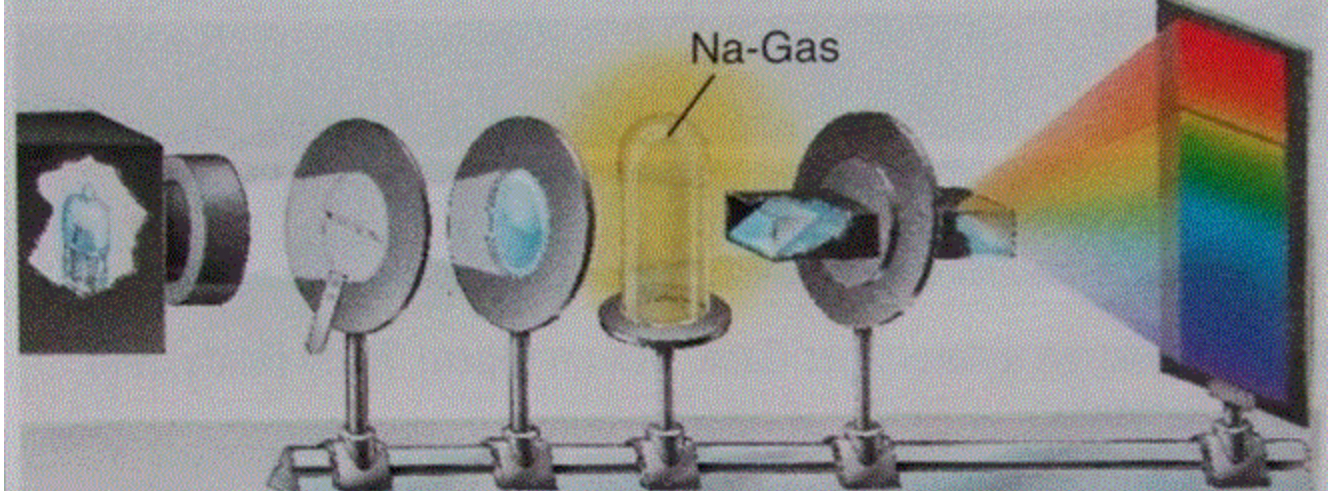
\includegraphics[width = 8cm]{graphics/IMG_0920.PNG}
    \end{center}
	
\end{enumerate}
Man spricht von der quantenhaften Abssorption von Licht. Dabei erhält man ein Absorptionsspektrum. Das Absorptionsspektrum eines Stoffes enthält dunkle Linien, die der Stoff im weißen Glühlicht absorbiert.\\\\
Das Sonnenspektrum weist schwarze Linien auf, die nach ihrem Entdecker \textit{frauhofersche Linien} heißen.\\
Sie liegen bei Frequenzen, die sich auch in den Emissionsspektren einiger elemente wiederfinden lassen. Diese Elemente in der sonnenatmosphäre verursachen durch die Absorption von Lichtquanten bestimmter Frequenzen diese dunklen Linien, sodass sie im kontinuierlichen Spektrum des Sonnenlichts fehlen.
\subsection{Exkurs: Entwicklung des Atommodells}
\label{sec:Exkurs: Entwicklung des Atommodells}
\begin{itemize}
  \item \textit{Demokrit 460-370 v. Chr.:}	\\
    -Atome sind unteilbare Teilchen, aus denen alles besteht
  \item \textit{Dalton, 1766-1844:}	\\
    -Atome sind elastische Kugeln mit einer bestimmten Masse\\
    -unterschiedliche Elemente haben Atome mit unterschiedlicher Masse
  \item \textit{Balmer, 1885}	\\ 
    \textbf{Balmer Formel:}	$f_{m, 2} = R\cdot  (\frac{1}{2^{2}}-\frac{1}{m^{2}}		)$
  \item \textit{Thomsom, 1903:}	"Rosinenkuchenmodell":\\
    -negative Elektronen sind in positiver Masse "eingebettet"
  \item \textit{Rutherford, 1911:}	 Alpha-Streuversuch\\
    -Atome können keine massiven Kugeln sein\\
    -Atom besteht aus massivem Kern und einer Hülle (Grössenverältnis 1: 100.000)

 \end{itemize}
\end{document}
